\documentclass{article}

\usepackage{tabularx}
\newcolumntype{L}[1]{>{\raggedright\arraybackslash}p{#1}} % linksbündig mit Breitenangabe
\newcolumntype{C}[1]{>{\centering\arraybackslash}p{#1}} % zentriert mit Breitenangabe
\newcolumntype{R}[1]{>{\raggedleft\arraybackslash}p{#1}} % rechtsbündig mit Breitenangabe

\usepackage{graphicx}
\usepackage{amsmath,amssymb,amsfonts,amsthm,mathtools} % Mathematik
\usepackage{subfigure} 
\usepackage{color}

\usepackage{pdfpages}

\usepackage[top=1.5cm, bottom=1.5cm]{geometry}

\usepackage{caption}

\title{Sheet 4 - Answers}
\author{Timm \& Boris}

\begin{document}
\maketitle

\section*{Task: 1}
Plot for the integrand of a two-dimensional Down-Out Call option with barrier B.
\begin{figure}[htbp]
  \centering
     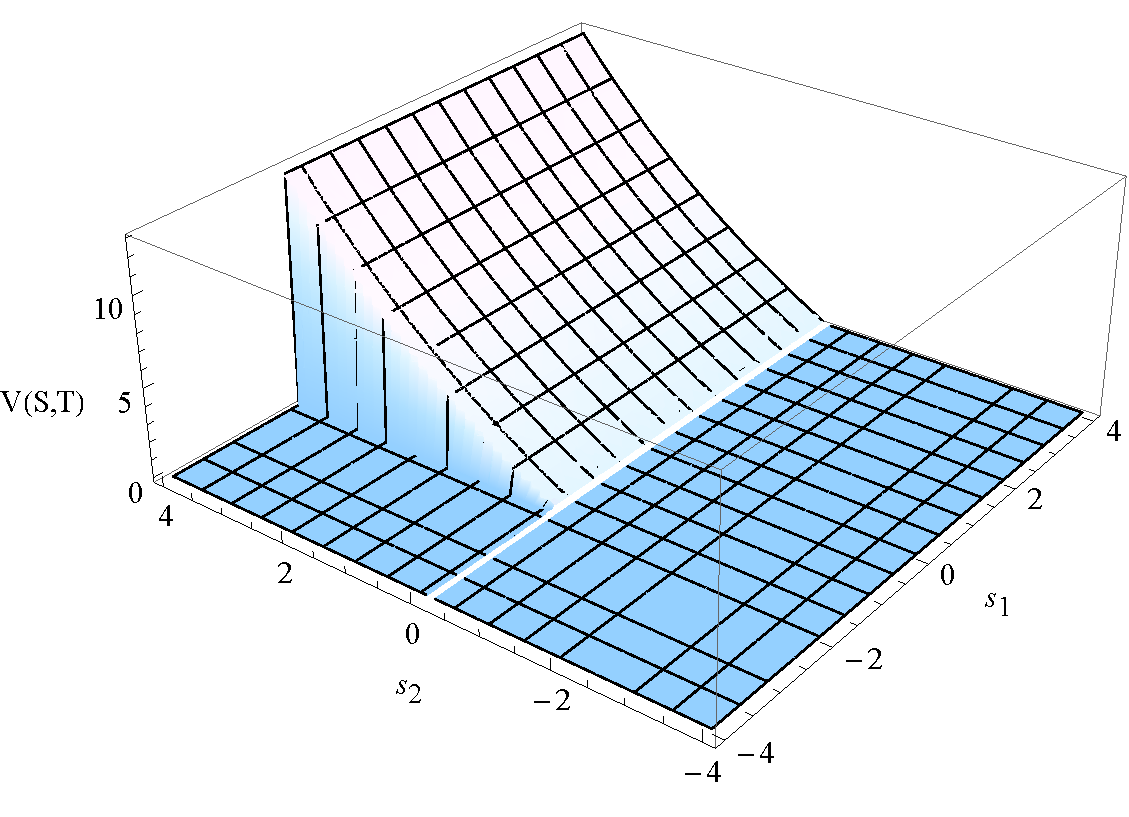
\includegraphics[width=1.0\textwidth]{../Task01/task01_plot.pdf}
  \caption*{Integrand of 2-dimensional Down-Out Call option.}
\end{figure}

\section*{Task: 2}
\subsection*{Part 1}
Convergence Plot of a Brownian Bridge and Random Walk construction for a Barrier Down Out Call option with Monte Carlo and Quasi Monte Carlo.
\begin{figure}[htbp]
  \centering
     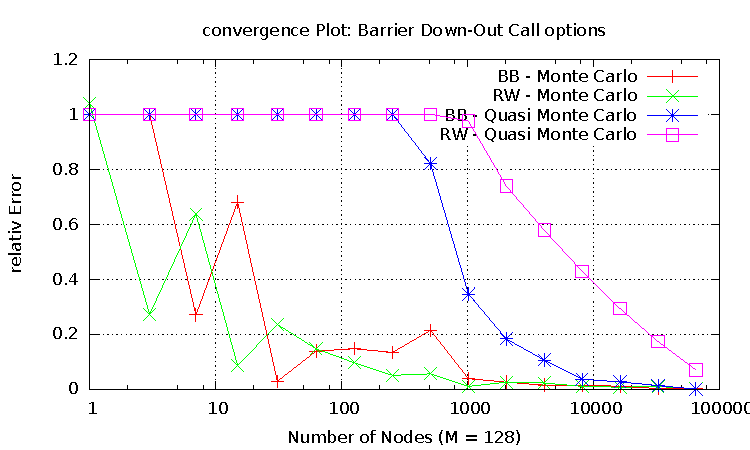
\includegraphics[width=1.0\textwidth]{../Task02/sh4_task02_convergencePlot.pdf}
%    \caption{}
\end{figure}

\subsection*{Part 2}
This Plot illustrates the error for a not sufficiently big reference value. Here is $ l \le 20 $, but the reference value is only $ l = 16 $.
\begin{figure}[htbp]
  \centering
     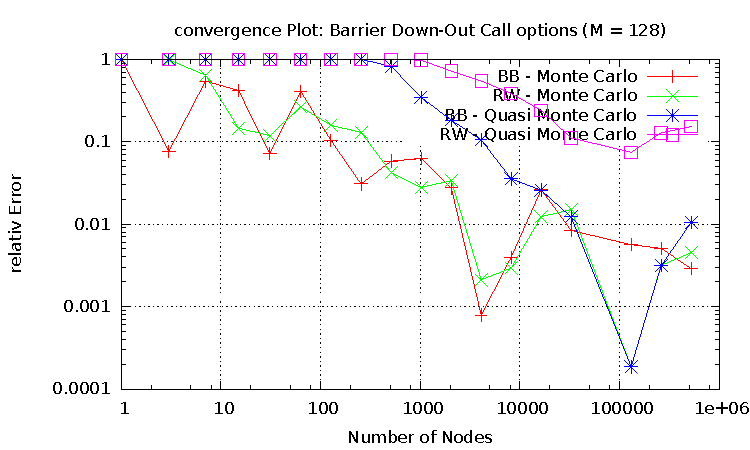
\includegraphics[width=1.0\textwidth]{../Task02/sh4_task02_2_convergencePlot.pdf}
%    \caption{}
\end{figure}
\newpage
This is an alternative, where the missing zero value for $ l = 16 $ is not left out.
\begin{figure}[htbp]
  \centering
     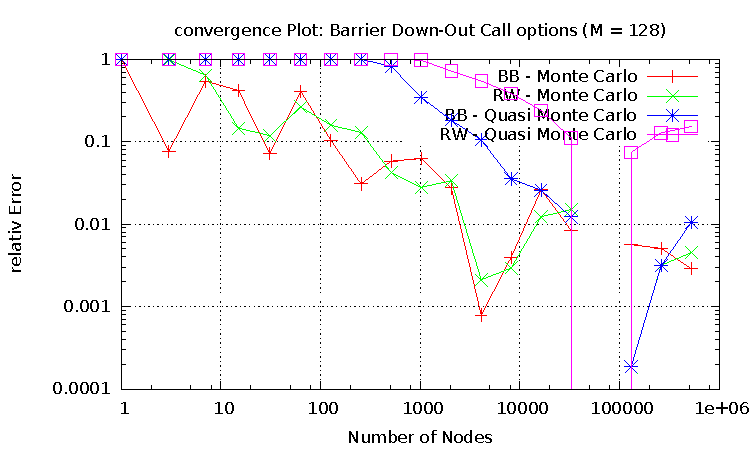
\includegraphics[width=1.0\textwidth]{../Task02/sh4_task02_2_alternativ.pdf}
%    \caption{}
\end{figure}

\section*{Task: 3}
Plot of the Black Scholes formula for a Down-Out call option.
\begin{figure}[htbp]
  \centering
     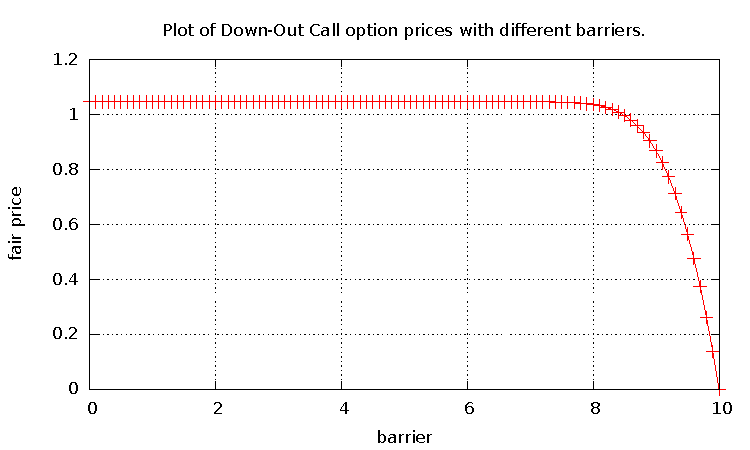
\includegraphics[width=1.0\textwidth]{../Task03/sh4_task3_price_plot.pdf}
%    \caption{}
\end{figure}

\section*{Task: 4}
This is also a convergence Plot of a Brownian Bridge and Random Walk construction for a Barrier Down Out Call option. But this time only for Monte Carlo (no QMC) and with different M = \{4, 64, 256, 1024\}.
 \begin{figure}[htbp]
	\begin{minipage}[b]{0.5\textwidth}
      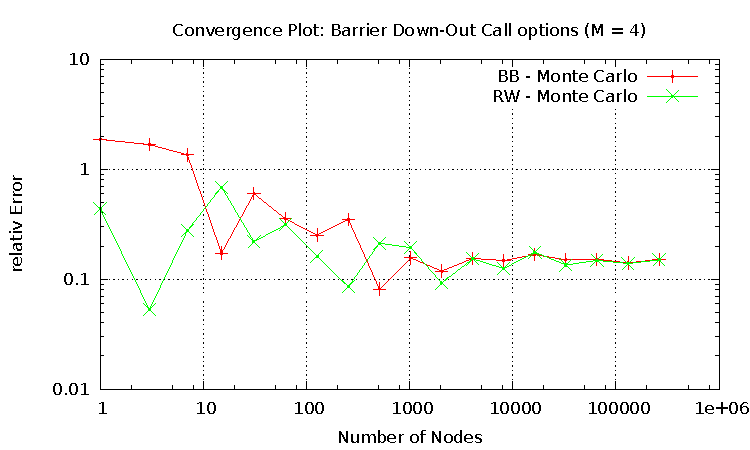
\includegraphics[width=1.0\textwidth]{../Task04/sh4_task04_convergencePlot_M=4.pdf}
    \end{minipage}
	\begin{minipage}[b]{0.5\textwidth}
   	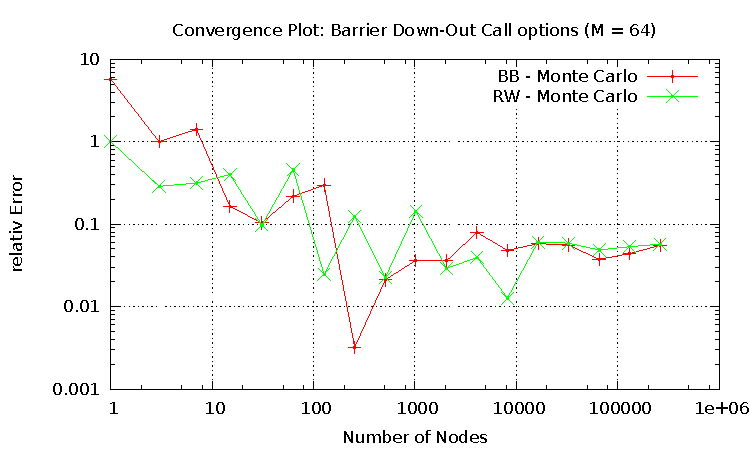
\includegraphics[width=1.0\textwidth]{../Task04/sh4_task04_convergencePlot_M=64.pdf}	
    \end{minipage}
  %    \caption{}
  \end{figure}
 \begin{figure}[htbp]
	\begin{minipage}[b]{0.5\textwidth}
      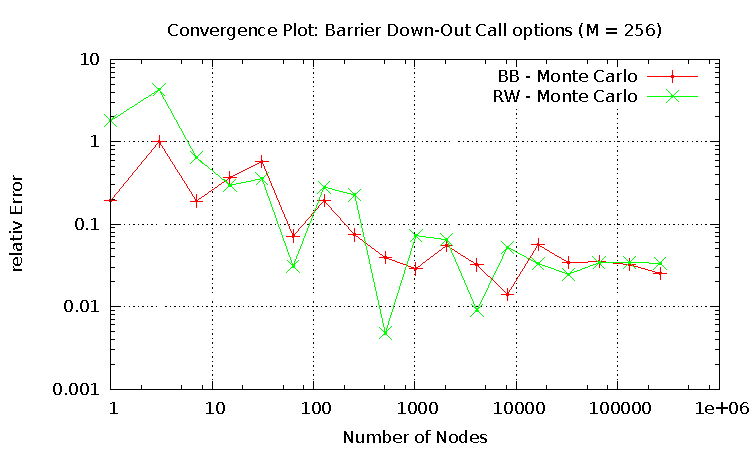
\includegraphics[width=1.0\textwidth]{../Task04/sh4_task04_convergencePlot_M=256.pdf}
    \end{minipage}
	\begin{minipage}[b]{0.5\textwidth}
   	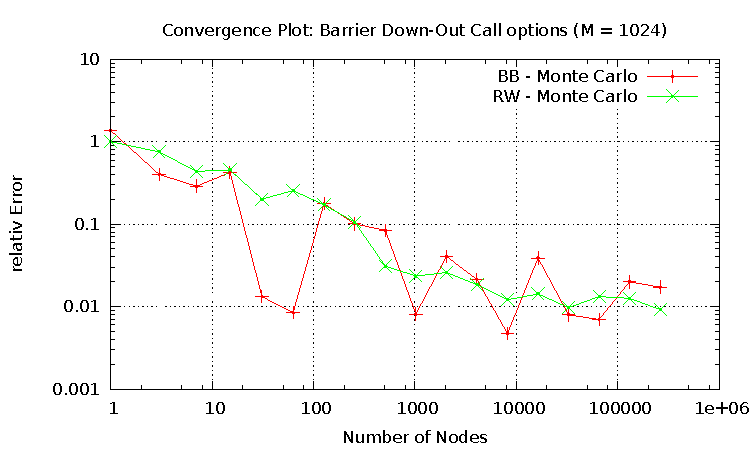
\includegraphics[width=1.0\textwidth]{../Task04/sh4_task04_convergencePlot_M=1024.pdf}	
    \end{minipage}
  %    \caption{}
  \end{figure}

\section*{Task: 5}
Plot of the discrete time integrand (for Lookback option with fixed strike) for M = 2 with the usual parameters.
\begin{figure}[htbp]
  \centering
     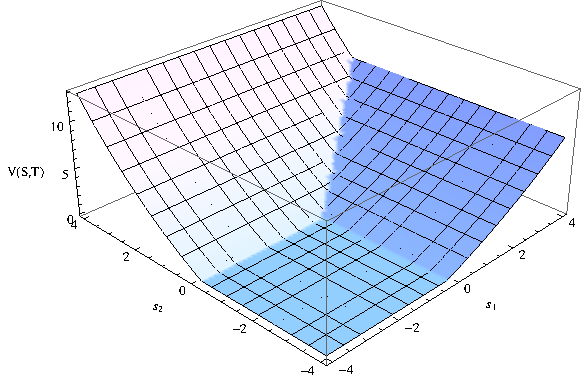
\includegraphics[width=0.8\textwidth]{../Task05/task05_plot.pdf}
%    \caption{}
\end{figure}

\newpage
\section*{Task: 6}
This is a convergence plot for for MC and QMC for a discrete time Lookback option with M = 128. The path discretization is done with Brownian Bridge.

\begin{figure}[htbp]
  \centering
     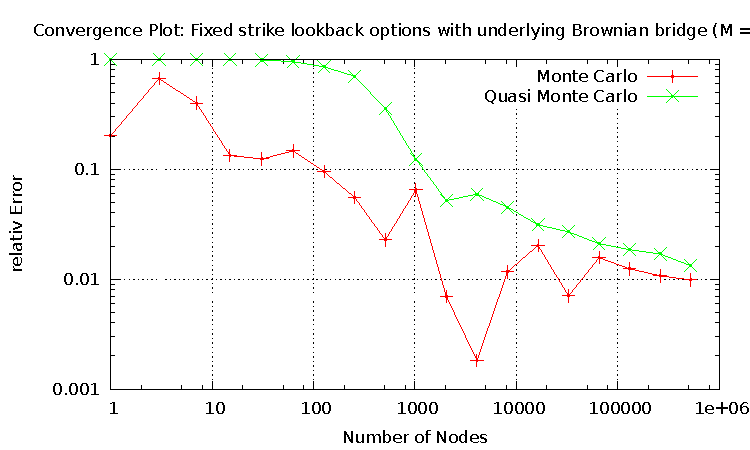
\includegraphics[width=0.8\textwidth]{../Task06/sh4_task06_convergencePlot.pdf}
%    \caption{}
\end{figure}
\section*{Task: 7}
Call option implied volatilities computed with Newton-Raphson algorithm with different start values $\sigma_0$ and for different actual $\sigma$ ($2 V / (\sqrt{T} S(0)) = 0.0975412$):% for computing the implied volatility:
\begin{table}[htbp]%[tphp]
  \centering
  \renewcommand{\arraystretch}{1}
  \renewcommand{\tabcolsep}{0.25em} 
%   \scalebox{1.0}{
%   \ttfamily
  \begin{tabular}{p{2.0cm}|| R{1.6cm} |R{1.6cm} |R{1.6cm} |R{1.6cm} |R{1.6cm} }
%     \rowstyle{\bfseries}

actual $\sigma$ \textbackslash $\sigma_0$  & 0.0975412 & 0.0100000 & 1.0000000 &10.0000000 & 0.1000000\\
           \hline
           \hline
 0.0010000 & 0.0091670 & 0.0091670 &       nan &       nan & 0.0091670 \\
 0.0100000 & 0.0100000 & 0.0100000 &       nan &       nan & 0.0100000 \\
 1.0000000 & 1.0000000 &       nan & 1.0000000 &       nan & 1.0000000 \\
 9.0000000 & 9.0000000 &       nan & 9.0000000 & 9.0000000 & 9.0000000 

  \end{tabular}
%   \large
%   \caption*{}

\end{table}

Put option implied volatilities computed with Newton-Raphson algorithm with different start values $\sigma_0$ and for different actual $\sigma$ ($2 V / (\sqrt{T} S(0)) = 0$): 
\begin{table}[htbp]%[tphp]
  \centering
  \renewcommand{\arraystretch}{1}
  \renewcommand{\tabcolsep}{0.25em} 
%   \scalebox{1.0}{
%   \ttfamily
  \begin{tabular}{p{2.0cm}|| R{1.6cm} |R{1.6cm} |R{1.6cm} |R{1.6cm} |R{1.6cm} }
%     \rowstyle{\bfseries}

actual $\sigma$ \textbackslash $\sigma_0$ & 0.0000000 & 0.0100000 & 1.0000000 &10.0000000 & 0.1000000\\
           \hline
           \hline
 0.0010000 & 0.0091670 & 0.0091670 &       nan &       nan & 0.0091670 \\
 0.0100000 & 0.0100000 & 0.0100000 &       nan &       nan & 0.0100000 \\
 1.0000000 & 1.0000000 &       nan & 1.0000000 &       nan & 1.0000000 \\
 9.0000000 & 9.0000000 &       nan & 9.0000000 & 9.0000000 & 9.0000000 
  \end{tabular}
%   \large
%   \caption*{}

\end{table}

One observed cause for the divergence of the algorithm is that the quotient $\sigma_0 / \sigma$ diverges too far from one (either is too large or too near to zero).

% \section*{Task: 8}

\newpage
\section*{Task: 9}
We looked up some values from "{}www.onvista.de"{}. % and made screenshots of the entries we used. 
We used values of a Gold stock and European call options of UBS with same time of maturity.% and for European options.
One can observe the smile and one runaway value.
\begin{figure}[htbp]
  \centering
     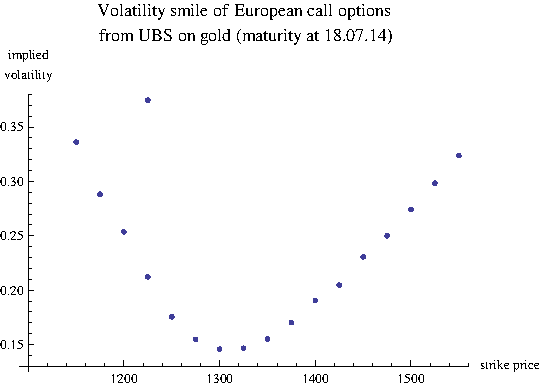
\includegraphics[width=1.0\textwidth]{../Task09/smileFromExternalData.pdf}
%    \caption{}
\end{figure}


\end{document}